\documentclass[tikz,border=10pt]{standalone}
\usepackage{mathabx}
\usepackage{stackengine}
\usetikzlibrary{backgrounds}
\usepackage{newunicodechar}
\newunicodechar{♮}{$\natural$}
\newunicodechar{♭}{$\flat$}
\newunicodechar{♯}{$\sharp$}
\newunicodechar{➚}{$\nearrow$}
\newunicodechar{➘}{$\searrow$}
\newunicodechar{ʼ}{'}
\newunicodechar{Ȧ}{\stackon[0.8pt]{A}{.}}
\newunicodechar{Ḃ}{\stackon[0.8pt]{B}{.}}
\newunicodechar{Ċ}{\stackon[0.8pt]{C}{.}}
\newunicodechar{Ḋ}{\stackon[0.8pt]{D}{.}}
\newunicodechar{Ė}{\stackon[0.8pt]{E}{.}}
\newunicodechar{Ḟ}{\stackon[0.8pt]{F}{.}}
\newunicodechar{Ġ}{\stackon[0.8pt]{G}{.}}


\def\centerarc[#1](#2)(#3:#4:#5);%
{
  \draw[#1]([shift=(#3:#5)]#2) arc (#3:#4:#5);
}


\begin{document}
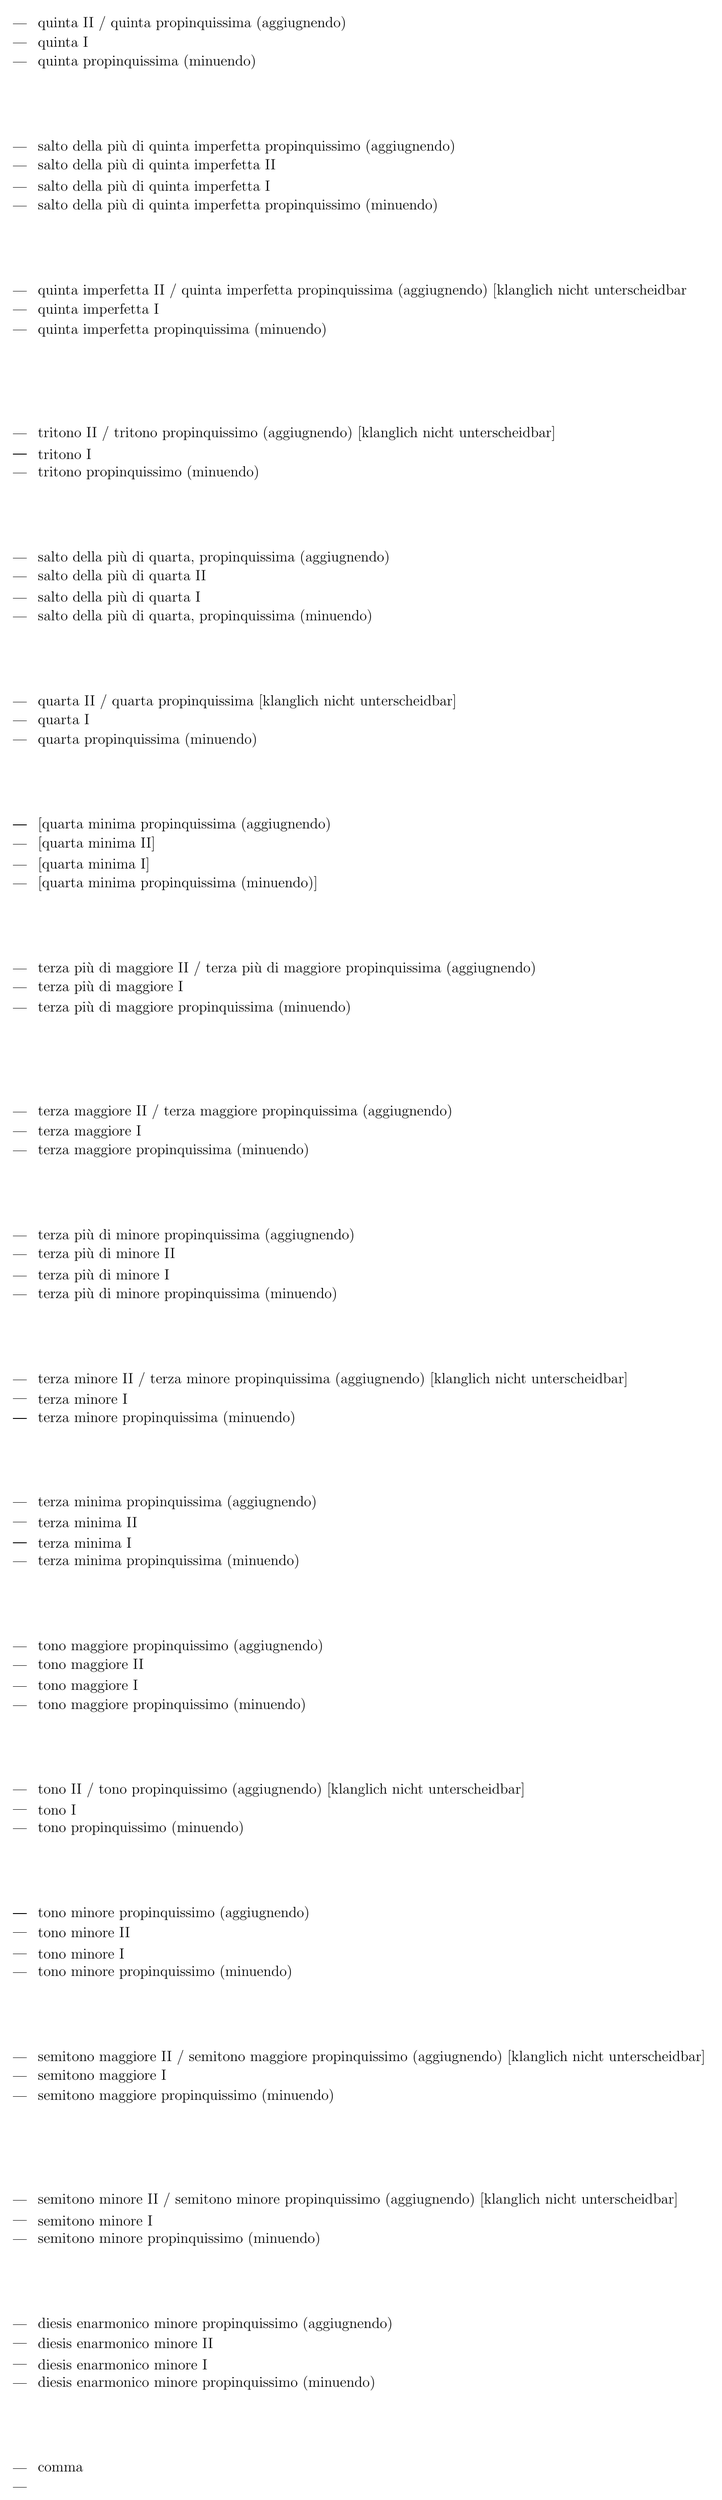
\begin{tikzpicture}

\node[anchor=west] at (484.1926, 0.5376352) { \large comma };
\node[anchor=west] at (484.1926, 2.961337) { \large diesis enarmonico minore propinquissimo (minuendo) };
\node[anchor=west] at (484.1926, 3.5045712) { \large diesis enarmonico minore I };
\node[anchor=west] at (484.1926, 4.105718) { \large diesis enarmonico minore II };
\node[anchor=west] at (484.1926, 4.643354) { \large diesis enarmonico minore propinquissimo (aggiugnendo) };
\node[anchor=west] at (484.1926, 7.0670533) { \large semitono minore propinquissimo (minuendo) };
\node[anchor=west] at (484.1926, 7.6049266) { \large semitono minore I };
\node[anchor=west] at (484.1926, 8.182639) { \large semitono minore II / semitono minore propinquissimo (aggiugnendo) [klanglich nicht unterscheidbar] };
\node[anchor=west] at (484.1926, 11.140228) { \large semitono maggiore propinquissimo (minuendo) };
\node[anchor=west] at (484.1926, 11.710625) { \large semitono maggiore I };
\node[anchor=west] at (484.1926, 12.248046) { \large semitono maggiore II / semitono maggiore propinquissimo (aggiugnendo) [klanglich nicht unterscheidbar] };
\node[anchor=west] at (484.1926, 14.672156) { \large tono minore propinquissimo (minuendo) };
\node[anchor=west] at (484.1926, 15.209842) { \large tono minore I };
\node[anchor=west] at (484.1926, 15.81626) { \large tono minore II };
\node[anchor=west] at (484.1926, 16.353764) { \large tono minore propinquissimo (aggiugnendo) };
\node[anchor=west] at (484.1926, 18.777876) { \large tono propinquissimo (minuendo) };
\node[anchor=west] at (484.1926, 19.315453) { \large tono I };
\node[anchor=west] at (484.1926, 19.873009) { \large tono II / tono propinquissimo (aggiugnendo) [klanglich nicht unterscheidbar] };
\node[anchor=west] at (484.1926, 22.276434) { \large tono maggiore propinquissimo (minuendo) };
\node[anchor=west] at (484.1926, 22.829899) { \large tono maggiore I };
\node[anchor=west] at (484.1926, 23.421097) { \large tono maggiore II };
\node[anchor=west] at (484.1926, 23.95886) { \large tono maggiore propinquissimo (aggiugnendo) };
\node[anchor=west] at (484.1926, 26.382563) { \large terza minima propinquissima (minuendo) };
\node[anchor=west] at (484.1926, 26.920439) { \large terza minima I };
\node[anchor=west] at (484.1926, 27.506683) { \large terza minima II };
\node[anchor=west] at (484.1926, 28.064161) { \large terza minima propinquissima (aggiugnendo) };
\node[anchor=west] at (484.1926, 30.463715) { \large terza minore propinquissima (minuendo) };
\node[anchor=west] at (484.1926, 31.026123) { \large terza minore I };
\node[anchor=west] at (484.1926, 31.563553) { \large terza minore II / terza minore propinquissima (aggiugnendo) [klanglich nicht unterscheidbar] };
\node[anchor=west] at (484.1926, 33.98777) { \large terza più di minore propinquissima (minuendo) };
\node[anchor=west] at (484.1926, 34.525326) { \large terza più di minore I };
\node[anchor=west] at (484.1926, 35.13175) { \large terza più di minore II };
\node[anchor=west] at (484.1926, 35.66927) { \large terza più di minore propinquissima (aggiugnendo) };
\node[anchor=west] at (484.1926, 38.093487) { \large terza maggiore propinquissima (minuendo) };
\node[anchor=west] at (484.1926, 38.630947) { \large terza maggiore I };
\node[anchor=west] at (484.1926, 39.19899) { \large terza maggiore II / terza maggiore propinquissima (aggiugnendo) };
\node[anchor=west] at (484.1926, 42.15672) { \large terza più di maggiore propinquissima (minuendo) };
\node[anchor=west] at (484.1926, 42.736595) { \large terza più di maggiore I };
\node[anchor=west] at (484.1926, 43.27447) { \large terza più di maggiore II / terza più di maggiore propinquissima (aggiugnendo) };
\node[anchor=west] at (484.1926, 45.698174) { \large [quarta minima propinquissima (minuendo)] };
\node[anchor=west] at (484.1926, 46.236034) { \large [quarta minima I] };
\node[anchor=west] at (484.1926, 46.832874) { \large [quarta minima II] };
\node[anchor=west] at (484.1926, 47.38) { \large [quarta minima propinquissima (aggiugnendo) };
\node[anchor=west] at (484.1926, 49.79652) { \large quarta propinquissima (minuendo) };
\node[anchor=west] at (484.1926, 50.341625) { \large quarta I };
\node[anchor=west] at (484.1926, 50.87916) { \large quarta II / quarta propinquissima [klanglich nicht unterscheidbar] };
\node[anchor=west] at (484.1926, 53.303528) { \large salto della più di quarta, propinquissima (minuendo) };
\node[anchor=west] at (484.1926, 53.841045) { \large salto della più di quarta I };
\node[anchor=west] at (484.1926, 54.4472) { \large salto della più di quarta II };
\node[anchor=west] at (484.1926, 54.984882) { \large salto della più di quarta, propinquissima (aggiugnendo) };
\node[anchor=west] at (484.1926, 57.40924) { \large tritono propinquissimo (minuendo) };
\node[anchor=west] at (484.1926, 57.946667) { \large tritono I };
\node[anchor=west] at (484.1926, 58.522144) { \large tritono II / tritono propinquissimo (aggiugnendo) [klanglich nicht unterscheidbar] };
\node[anchor=west] at (484.1926, 61.478237) { \large quinta imperfetta propinquissima (minuendo) };
\node[anchor=west] at (484.1926, 62.052223) { \large quinta imperfetta I };
\node[anchor=west] at (484.1926, 62.589565) { \large quinta imperfetta II / quinta imperfetta propinquissima (aggiugnendo) [klanglich nicht unterscheidbar };
\node[anchor=west] at (484.1926, 65.01394) { \large salto della più di quinta imperfetta propinquissimo (minuendo) };
\node[anchor=west] at (484.1926, 65.5517) { \large salto della più di quinta imperfetta I };
\node[anchor=west] at (484.1926, 66.15785) { \large salto della più di quinta imperfetta II };
\node[anchor=west] at (484.1926, 66.69528) { \large salto della più di quinta imperfetta propinquissimo (aggiugnendo) };
\node[anchor=west] at (484.1926, 69.11965) { \large quinta propinquissima (minuendo) };
\node[anchor=west] at (484.1926, 69.65727) { \large quinta I };
\node[anchor=west] at (484.1926, 70.20864) { \large quinta II / quinta propinquissima (aggiugnendo) };
\draw (483.99258,0.0) -- (483.5926,0.0);
\draw (483.99258,0.5376352) -- (483.5926,0.5376352);
\draw (483.99258,2.961337) -- (483.5926,2.961337);
\draw (483.99258,3.5045712) -- (483.5926,3.5045712);
\draw (483.99258,4.105718) -- (483.5926,4.105718);
\draw (483.99258,4.643354) -- (483.5926,4.643354);
\draw (483.99258,7.0670533) -- (483.5926,7.0670533);
\draw (483.99258,7.6049266) -- (483.5926,7.6049266);
\draw (483.99258,8.182639) -- (483.5926,8.182639);
\draw (483.99258,11.140228) -- (483.5926,11.140228);
\draw (483.99258,11.710625) -- (483.5926,11.710625);
\draw (483.99258,12.248046) -- (483.5926,12.248046);
\draw (483.99258,14.672156) -- (483.5926,14.672156);
\draw (483.99258,15.209842) -- (483.5926,15.209842);
\draw (483.99258,15.81626) -- (483.5926,15.81626);
\draw (483.99258,16.353764) -- (483.5926,16.353764);
\draw (483.99258,18.777876) -- (483.5926,18.777876);
\draw (483.99258,19.315453) -- (483.5926,19.315453);
\draw (483.99258,19.873009) -- (483.5926,19.873009);
\draw (483.99258,22.276434) -- (483.5926,22.276434);
\draw (483.99258,22.829899) -- (483.5926,22.829899);
\draw (483.99258,23.421097) -- (483.5926,23.421097);
\draw (483.99258,23.95886) -- (483.5926,23.95886);
\draw (483.99258,26.382563) -- (483.5926,26.382563);
\draw (483.99258,26.920439) -- (483.5926,26.920439);
\draw (483.99258,27.506683) -- (483.5926,27.506683);
\draw (483.99258,28.064161) -- (483.5926,28.064161);
\draw (483.99258,30.463715) -- (483.5926,30.463715);
\draw (483.99258,31.026123) -- (483.5926,31.026123);
\draw (483.99258,31.563553) -- (483.5926,31.563553);
\draw (483.99258,33.98777) -- (483.5926,33.98777);
\draw (483.99258,34.525326) -- (483.5926,34.525326);
\draw (483.99258,35.13175) -- (483.5926,35.13175);
\draw (483.99258,35.66927) -- (483.5926,35.66927);
\draw (483.99258,38.093487) -- (483.5926,38.093487);
\draw (483.99258,38.630947) -- (483.5926,38.630947);
\draw (483.99258,39.19899) -- (483.5926,39.19899);
\draw (483.99258,42.15672) -- (483.5926,42.15672);
\draw (483.99258,42.736595) -- (483.5926,42.736595);
\draw (483.99258,43.27447) -- (483.5926,43.27447);
\draw (483.99258,45.698174) -- (483.5926,45.698174);
\draw (483.99258,46.236034) -- (483.5926,46.236034);
\draw (483.99258,46.832874) -- (483.5926,46.832874);
\draw (483.99258,47.38) -- (483.5926,47.38);
\draw (483.99258,49.79652) -- (483.5926,49.79652);
\draw (483.99258,50.341625) -- (483.5926,50.341625);
\draw (483.99258,50.87916) -- (483.5926,50.87916);
\draw (483.99258,53.303528) -- (483.5926,53.303528);
\draw (483.99258,53.841045) -- (483.5926,53.841045);
\draw (483.99258,54.4472) -- (483.5926,54.4472);
\draw (483.99258,54.984882) -- (483.5926,54.984882);
\draw (483.99258,57.40924) -- (483.5926,57.40924);
\draw (483.99258,57.946667) -- (483.5926,57.946667);
\draw (483.99258,58.522144) -- (483.5926,58.522144);
\draw (483.99258,61.478237) -- (483.5926,61.478237);
\draw (483.99258,62.052223) -- (483.5926,62.052223);
\draw (483.99258,62.589565) -- (483.5926,62.589565);
\draw (483.99258,65.01394) -- (483.5926,65.01394);
\draw (483.99258,65.5517) -- (483.5926,65.5517);
\draw (483.99258,66.15785) -- (483.5926,66.15785);
\draw (483.99258,66.69528) -- (483.5926,66.69528);
\draw (483.99258,69.11965) -- (483.5926,69.11965);
\draw (483.99258,69.65727) -- (483.5926,69.65727);
\draw (483.99258,70.20864) -- (483.5926,70.20864);
\end{tikzpicture}
\end{document}